% Set document properties as required by FEKT specification
\documentclass[a4paper, 12pt]{article}
\usepackage[left=3cm,right=2cm,top=4cm]{geometry}

% Local settings
\usepackage[utf8x]{inputenc} 
\usepackage[czech]{babel}
\usepackage[IL2]{fontenc}
\usepackage{caption}
\usepackage{afterpage}
\usepackage{amsthm}
\usepackage{graphicx}
\usepackage{amsmath}
\usepackage{amsfonts}
\usepackage{fancyvrb}
\usepackage{hyperref}
\usepackage{pdfpages}
\hypersetup{
    colorlinks,
    citecolor=black,
    filecolor=black,
    linkcolor=black,
    urlcolor=black
}

% Set line spacing for whole document (sadly)
\renewcommand{\baselinestretch}{1.5}

% Helper commands
\providecommand{\uv}[1]{\quotedblbase #1\textquotedblleft}
\newcommand\textbox[1]{%
    \parbox{.5\textwidth}{#1}%
}

% Thesis variables
%\newcommand{\thesisName}{Implementace kybernetické bezpečnosti do ŠVP pro Informatiku a výpočetní techniku na gymnáziích}
\newcommand{\thesisName}{Implementace tématu kybernetické bezpečnosti do výuky předmětu Informatika a Výpočetní Technika pro gymnázia}
\newcommand{\universityName}{VYSOKÉ~~~UČENÍ~~~TECHNICKÉ~~~V~BRNĚ}
\newcommand{\facultyName}{Fakulta elektrotechniky a komunikačních technologií}
\title{\thesisname}
\author{Bc. Daniel Dušek}
\begin{document}

% === FRONT PAGE ===
\thispagestyle{empty}
\newgeometry{left=2cm,right=2cm,top=1.5cm}
    \begin{center}
        \Huge
        \universityName \\
            \vspace{\stretch{0.150}}
        
        \LARGE
        \textsc{\facultyName\\}
            \vspace{\stretch{0.300}}
        
        \Large{Závěrečná práce doplňujícího pedagogického studia \\ ~ \\}
        
        \LARGE
        \textsc{\thesisName}
            \vspace{\stretch{0.618}}
    \end{center}

        % Author and date part        
        \noindent \textbox{\today}  \textbox{\hfill \textbf{Vedoucí práce}: PhDr. Petra Fiľová} \\
        \noindent \textbox{\hfill}  \textbox{\hfill \textbf{Autor práce}: Bc. Daniel Dušek ~~~~~}
\clearpage
\restoregeometry

% === TABLE OF CONTENTS ===
\newpage
\thispagestyle{empty}
\setcounter{tocdepth}{2}
\tableofcontents

% === SECTION INTRODUCTION ===
\newpage
\setcounter{page}{1}
\section{Úvod}

Stejně jako bylo devatenácté století nazývané stoletím páry a dvacáté století stoletím techniky, bude jednou pravděpodobně dvacáté první století nazývané stoletím počítačů a sítí. Oblast techniky a informačních technologií se rozvíjí neustále vyšší a vyšší rychlostí, dostupnost \uv{chytré} elektroniky se zvyšuje tempem podobným. Společně s technikou a její vyšší dostupností se však objevuje další, bohužel nepříjemný fenomén -- a sice zneužívání technologií a jejich vysoké dostupnosti k páchání trestné činnosti. 

Trend zneužívání technologií a nedostatečné vzdělanosti v oblasti počítačové bezpečnosti lidí s nimi pracujících roste s každým rokem více a více. Útoky související s distribucí, v době psaní práce velmi populárního škodlivého software, zvaného ransomware vzrostly v počtu od roku 2015 neuvěřitelných 300$\%$.

Na jednu stranu možná i uklidňujícím faktem je, že v případě ransomware jsou cílem typicky organizace, nikoliv jednotlivci. Bohužel i v tomto případě se často obětí stane právě i jednotlivec, a to zejména díky způsobu, kterým se ransomware a jemu podobné škodlivé programy šíří. Jedním z častých scénářů je případ, kdy je počítač infikován prostřednictvím nakaženého souboru typu .xls(x), .doc(x), .ppt(x) apod., tedy soubory běžně produkované nástroji sady Microsoft Office. Druhým, opět velmi častým scénářem je pak případ, kdy se škodlivý soubor pouze tváří být souborem dříve jmenovaných typů, avšak ve skutečnosti je souborem úplně jiného typu, obsahujícího škodlivý kód. V obou dvou scénářích je klíčové, aby ovšem pochybil lidský článek pracující s takovýmto souborem. Tomuto pochybení by bylo poměrně snadné předcházet, a to vyšším obecným povědomím o tom jak správně a bezpečně pracovat s počítačem a internetem. 

Tohoto obecně vyššího povědomí by bylo možné dosáhnout například kladením vyššího důrazu na výuku kybernetické bezpečnosti ve školách v rámci výuky informačních technologií, výpočetní techniky a informatiky. V konkrétních termínech například místo kladení obrovského důrazu pouze na výuku práce s nástroji kancelářského balíku Microsoft Office slevit lehce z časové dotace vyhrazené na vysvětlování funkcionality a následné zkoušení žáků z ní, a tuto časovou úsporu věnovat k osvětlování způsobů a principů, kterými jsou soubory balíku Microsoft Office zneužívány hackery pro napadení počítačů a způsobů obrany a bezpečné práce s těmito soubory. Snížení časové dotace na vysvětlování a zkoušení funkcionality by, dle autora této práce, nemuselo mít vyloženě negativní dopad, neboť většina dnešní generace přichází do styku s počítači a těmito programy na denní bázi. Navíc jsou tyto programy v posledních letech průběžně neustále vylepšovány z hlediska uživatelské přívětivosti, aby práce s nimi byla více intuitivní a snadná. 

Dalším důvodem pro zavedení výuky kybernetické bezpečnosti do osnov je zcela opačný pól kybernetické bezpečnosti. Doposud bylo psáno hlavně o způsobech ochrany a osvěty běžných uživatelů výpočetní techniky proti útokům ze strany hackerů. Stejně, ne-li více důležitou částí výuky kybernetické bezpečnosti by měla být osvěta žáků o možných následcích zneužívání výpočetní techniky k páchání trestných činů. Mezi studenty se vyskytuje dnes již poměrně veliká část žáků, která je seznámena s prací s počítačem natolik, že je potenciálně schopná počítač i nějakým způsobem programovat. Někteří z těchto žáků mohou potřebovat vyjasnit fakt, že existuje hranice, za níž nesmí při programování svých aplikací zajít. Ačkoliv se to může zdát z prvního pohledu jako celkem jednoduchá otázka k diskusi, nemusí to vždy být pravda. Konkrétním případem může být 16 letý chlapec Ashkan Hosseini, jenž naprogramoval aplikaci, kterou nahrál na CD s rodinnými fotkami~\cite{malwareUnicornAppretince}. Aplikace následně způsobila, že po strčení CD do počítače došlo k vymazání všech rodinných fotek jak z CD, tak z počítače, do kterého bylo CD zastrčeno. Ashkan naprogramoval tuto aplikaci za účelem odstranění fotek na kterých se nacházel -- jeho úmysly tedy nebyly vyloženě špatné a díky tomu, že CD putovalo pouze mezi rodinou, Ashkan nebyl nikým žalován. Pokud by se ale stalo, že by jeho aplikace unikla do světa a napadla cizí počítač, dopustil by se již vážného trestného činu, aniž by si tyto následky svých akcí uvědomil. V Americe by to pro něho pak mohlo znamenat až 5 let vězení. Příběh Ashkana Hosseiniho dopadl tedy naštěstí pro něho dobře, kde navíc jeho rodiče měli dostatek reflexe a nabídli mu možnost studovat oblast boje proti kybernetické kriminalitě, které se chopil. Ne všichni žáci však musí vždy přesně odlišit hranici toho, kdy končí \uv{legrace} a začíná páchání trestného činu, alespoň ne v oblasti počítačů a sítí, a ne všichni musí mít to štěstí, jaké Ashkan měl. I z tohoto důvodu je třeba šířit povědomí o kybernetické bezpečnosti a implikacích, které může mít na život jedince nedodržování jejích zásad. 

V letech 2007--2009 byla reakcí českého školství na prudký rozvoj a expanzi výpočetní techniky snaha naučit žáky a studenty s těmito novými technologiemi pracovat a interagovat. Tato snaha byla realizována v rámci vlnově vydávaných rámcově vzdělávacích programů -- dále jen RVP -- v nichž byl již povinně vyhrazen prostor pro výuku informačních a komunikačních technologií a informatiky~\cite{waveRVP}. Autor této práce považuje tuto reakci za dobře načasovanou a vhodnou. 

Nyní však nastává nová éra, kdy zařízení schopná připojení k Internetu jsou doslova i obrazně na každém našem kroku. Každé zařízení připojené k Internetu se může stát cílem útoku, stejně jako se obětí počítačové kriminality může stát každá osoba s těmito zařízeními pracující. Vzniká tedy takto nová potřeba většího důrazu na výuku těchto aspektů práce s informačními technologiemi. Tato práce má za cíl demonstrovat konkrétní možnou implementaci takové výuky do výuky ICT na gymnáziích.

% === DICTIONARY ===
% TODO: Zkontrolovat, že všechna problematická slova se vyskytují ve slovníčku pojmů.
\newpage
\section{Slovníček pojmů}
V textu této práce je možné se setkat s pojmy, které mají speciální význam v oblasti počítačové či kybernetické bezpečnosti, jenž se často liší od pocitového významu, který by si oblasti neznalý čtenář mohl vytvořit. Tato sekce si klade za cíl rozptýlit možné nejasnosti a mnohoznačnosti.

\textbf{Malware} -- Souhrné označení pro programy které vykonávají škodlivou činnost (trojské koně, viry, programy špehující uživatele, programy zobrazující uživateli nevyžádanou reklamu, a další).

\textbf{Škodlivý kód} -- Chce-li programátor přikázat počítači, aby vykonal nějakou činnost, popíše tuto činnost pomocí tzv. \textit{kódu}. Škodlivý kód je pak takový kód, který je-li vykonán počítačem, provede něco, co uživatel/majitel tohoto počítače nechce. Útočníci se při útoku snaží typicky právě vykonat škodlivý kód na zařízení, které napadají. Tento škodlivý kód bývá velmi často nastražen a ukryt tak, aby si uživatel pracující s počítačem vůbec neuvědomil, že kód spouští a vykonává.

\textbf{Nakažený soubor} -- Soubor v němž je kromě původního obsahu souboru navíc obsažen škodlivý kód. Škodlivý kód do souboru umístil buď přímo, nebo zprostředkovaně (například prostřednictvím škodlivého programu) útočník.

\textbf{Ransomware} -- Škodlivý program založený na principu držení rukojmí. Program po průniku do počítače zašifruje některé soubory, popřípadě uživateli úplně znemožní práci s počítačem. Za zpřístupnění souborů či zařízení je po uživateli požadováno zaplacení výkupného. Zaplacení výkupného nemusí vždy vést k získání objektu, který je držen jako rukojmí.

\textbf{Phishing} -- Typ útoku při kterém útočník předstírá, že je důvěryhodná, uživateli dobře známá entita, aby uživatele přiměl k vydání osobních či jinak citlivých informací a dat.


% === RVP & SVP CHAPTER ===
\newpage
\section{Výuka informatiky dle rámcového vzdělávacího programu a školního vzdělávacího programu}
Tato část práce se zabývá prostorem vyhrazeným pro výuku informatiky v rámci \textit{rámcového vzdělávacího programu} (dále jen RVP) a jeho možnou utilizací pro výuku kybernetické bezpečnosti. Dále je zde rozebrán konkrétní \textit{školní vzdělávací program} (dále jen ŠVP) v rámci něhož je vyhrazen prostor pro výuku informatiky. Dále v této kapitole je návrh rozšíření ŠVP tak, aby poskytoval dostatečný prostor k výuce kybernetické bezpečnosti. 

\subsection{Očekávané výstupy a cíle vzdělávání}
RVP pro gymnázia z roku 2007 uvádí následující cílové zaměření vzdělávací oblasti Informatiky a Informačních a komunikačních technologií~\cite{rvpGym}, která vedou žáka k:
\begin{itemize}
    \setlength{\itemsep}{-3pt}
    \item porozumění zásadám ovládání a věcným souvislostem jednotlivých skupin aplikačního programového
vybavení a k vhodnému uplatňování jejich nástrojů, metod a vazeb k efektivnímu řešení úloh;
    \item porozumění základním pojmům a metodám informatiky jako vědního oboru a k jeho uplatnění
v ostatních vědních oborech a profesích;
    \item uplatňování algoritmického způsobu myšlení při řešení problémových úloh;
    \item využívání prostředků ICT k modelování a simulaci přírodních, technických a společenských procesů
a k jejich implementaci v různých oborech;
    \item tvořivému využívání spektra možností komunikačních technologií a jejich kombinací k rychlé
a efektivní komunikaci;
    \item využívání výpočetní techniky ke zvýšení efektivnosti své činnosti, k dokonalejší organizaci práce
a k týmové spolupráci na úrovni školní, republikové a mezinárodní;
    \item využívání informačních a komunikačních technologií (on-line vzdělávání, spolupráce na
zahraničních projektech) k celoživotnímu vzdělávání a vytváření pozitivních postojů k potřebám
znalostní společnosti;
    \item využití možností výpočetní techniky a internetu k poznávacím, estetickým a tvůrčím cílům s ohledem ke globálnímu a multikulturnímu charakteru internetu;
    \item \textbf{uvědomění si, respektování a zmírnění negativních vlivů moderních informačních a komunikačních technologií na společnost a na zdraví člověka, ke znalosti způsobů prevence a ochrany před zneužitím a omezováním osobní svobody člověka};
    \item \textbf{získávání údajů z většího počtu alternativních zdrojů a odlišování informačních zdrojů věrohodných a kvalitních od nespolehlivých a nekvalitních};
    \item respektování a používání odborné terminologie informačních a počítačových věd;
    \item \textbf{poznání základních právních aspektů a etických zásad týkajících se práce s informacemi a výpočetní technikou, k respektování duševního vlastnictví, copyrightu, osobních dat a zásad správného citování autorských děl}.
\end{itemize}

Výše zmíněné, zvýrazněné body jsou místa, které se více či méně dotýkají kybernetické bezpečnosti, a v rámci jejichž tématických záběrů je v této práci navrhována a implementována výuka kybernetické bezpečnosti v rámci výuky Informatiky a ICT na gymnáziích.
 
První ze tří zvýrazněných odstavců poskytuje prostor pro témata soustředící se na osvětu studentů v oblasti aktuálních hrozeb, které se ve světě kybernetické bezpečnosti vyskytují. Zmiňovaná osvěta má za cíl minimalizovat možný dopad těchto hrozeb na studenty, popřípadě jejich okolí. Konkrétní implementace výuky spadající pod prostor poskytovaný tímto bodem by v době psaní této práce mohla například zahrnovat látku diskutující kanály a způsoby, kterými je šířen \textit{ransomware}, který je velmi aktuální hrozbou, a to i především pro běžné uživatele počítače a Internetu. Dále pak také sadu tzv. \textit{dobrých zvyků}, jejichž aplikací je možné předejít infekci počítače tímto druhem škodlivého programu.

Druhý ze zvýrazněných odstavců vytváří prostor pro vzdělávání studentů ve správné práci s informačními zdroji. I zde je možné hledat spojitost s kybernetickou bezpečností. Tématicky by se zde daly diskutovat nebezpečí útoků cílených na konkrétní skupinu uživatelů, popřípadě na konkrétního uživatele -- jedince, které jsou založené na dezinformaci subjektu či \uv{prolamování} jednotlivce namísto počítačového systému. V době psaní práce by pod tímto bodem mohlo být vhodné rozvíjet výuku témat jako jsou \textbf{krádeže identity}, \textbf{sociální inženýrství}, či velmi populární \textbf{lživé zprávy} (pozn. v angličtině \textit{Fake news}).

Třetí zvýrazněný odstavec pak pod částí \uv{\textit{poznání základních právních aspektů a etických zásad týkajících se práce s informacemi a výpočetní technikou}} dává prostor pro vysvětlení možných právních následků pro jedince, kteří se rozhodnou zneužít znalost témat počítačové bezpečnosti k vlastnímu profitu na úkor druhých, tedy se postaví za \uv{hranu} zákona. Zahrnout lze i témata týkající se správného postupu při nalezení či získání důvěrné informace třetí strany, správného postupu při hlášení nalezených bezpečnostních chyb v lidských procesech, či aplikacích. Výuka pod tímto bodem by měla nabádat studenty k zodpovědnému chování a přístupu při práci s počítači, a to v souvislosti s kybernetickou bezpečností.


\subsection{Prostor vyhrazený v RVP pro gymnázia}
RVP pro gymnázia z roku 2007 předepisuje pro výuku Informatiky a ICT  minimální rozsah 4 hodiny týdně ve čtyřech letech s volitelným vyučováním v libovolném roce z 4 let. Bývá zvykem, že z hlediska ŠVP je toto realizováno výukou Informatiky a ICT po první dva roky v rozsahu 2 hodiny týdně (\textit{pozn. referenční ŠVP využité v této práci to má takto}). Dále je poskytnuto celkem 26 hodin \textit{disponibilní časové dotace}, ze kterých je možné při implementaci konkrétního ŠVP čerpat a výuku Informatiky a ICT rozšiřovat. Další možností je pak výuka Informatiky a ICT v 3. a 4. ročníku v rámci alokovaného času pro povinné \textit{Volitelné vzdělávací aktivity}, který je vyměřen na 8 hodin.

Autor této práce se domnívá, že vhodný způsob začlenění výuky kybernetické bezpečnosti do výuky by byla realizace samostatného předmětu \textit{Kybernetická bezpečnost} s využitím času vyhrazeného pro \textit{Volitelné vzdělávací aktivity}. Tento předmět by byl vyučován po dobu dvou let ve 3. a 4. ročníku, po tom, co studenti již absolvovali výuku Informatiky a ICT, na kterou by tento předmět navazoval. Umožnění studentům vybrat si \textit{Kybernetickou bezpečnost} jako volitelnou specializaci by teoreticky vedlo k vyučovacím třídám složeným ze studentů se zájmem o předmět bezpečnosti, kteří by se již během studia gymnázia mohli dále rozhodnout, zda chtějí pokračovat v kariéře v této perspektivní oblasti. Složení třídy ze zaujatých studentů by dále mohlo vést k svižnějšímu tempu výuky s větším důrazem na detail probíraného tématu, neb lze očekávat, že studenti se zájmem o kybernetickou bezpečnost zvládají práci s počítačem na dostatečné 
úrovni, a jsou namotivováni pracovat i mimo vyučovací hodiny.

Současně si je však autor této práce vědom, že momentálně ještě na gymnáziích neexistuje dostatečná potřeba vyučovat předměty týkající se přímo kybernetické bezpečnosti, pravděpodobně z toho důvodu, že kybernetická bezpečnost jako taková ještě není přímo zmiňována v RVP. Proto v rámci této práce je navrhován poněkud střízlivější způsob začlenění výuky kybernetické bezpečnosti do výuky na gymnáziích, a to formou doplňujících hodin ke standardní výuce Informatiky a ICT a zvýšením časové dotace pro její výuku.

\subsection{Rozbor konkrétního školního vzdělávacího programu}
Pro uvedení navrhované výuky kybernetické bezpečnosti do kontextu výuky Informatiky a ICT na gymnáziích se autor této práce rozhodl využít jako referenční případ existující školní vzdělávací program \textit{Gymnázia Boskovice}~\cite{svpGymbos}. Autor této práce prozkoumal více volně dostupných ŠVP pro různá gymnázia a došel k závěru, že v kontextu výuky Informatiky a ICT je Gymnázium Boskovice vhodným zástupcem pro reprezentaci třídy \uv{běžných gymnázií}. Z tohoto důvodu bylo vybráno právě toto ŠVP.

Rozložení hodin výuky v ŠVP je dáno na 2 hodiny týdně v prvních dvou ročnících a 0 hodin týdně pro třetí a čtvrtý ročník. V konkrétním ŠVP je ještě uvedeno dělení, kdy studenti oboru \textit{živé jazyky} mají sníženu dotaci o jednu hodinu týdně během prvních dvou let, avšak tato informace není pro kontext této práce relevantní a je uvažována dotace 2 hodiny týdně. Ve třetím a čtvrtém ročníku si pak studenti mohou ještě volitelně zvolit rozšiřující seminář Informatiky a Výpočetní techniky s dotací 5 hodin. Toto však také není přímo relevantní pro kontext této práce, neb typické gymnázium dotaci v této výši ne vždy uděluje.

Po absolvování výuky Informatiky a ICT na gymnáziu dle zkoumaného ŠVP splňují žáci všechny očekávané výstupy z oblastí daných RVP~\cite{rvpGym}:
\begin{itemize}
    \setlength{\itemsep}{-3pt}
    \item \textbf{Digitální technologie} - ovládá, propojuje a aplikuje dostupné prostředky ICT; využívá teoretické i praktické poznatky a o funkcích jednotlivých složek hardwaru a softwaru k tvůrčímu a efektivnímu řešení úloh; organizuje účelně data a chráni je proti poškození či zneužití; orientuje se v možnostech uplatnění ICT v různých oblastech společenského poznání a praxe.
    \item \textbf{Zdroje a vyhledávání informací, komunikace} - využívá dostupné služby informačních sítí k vyhledávání informací, ke komunikaci, k vlastnímu vzdělávání a týmové spolupráci; využívá nabídku informačních a vzdělávacích portálů, encyklopedií, knihoven, databází a výukových programů; posuzuje tvůrčím způsobem aktuálnost, relevanci a věrohodnost informačních zdrojů a informací; využívá informační a komunikační služby v souladu s etickými, bezpečnostními a legislativními požadavky.
    \item \textbf{Zpracování a prezentace informací} - zpracovává a prezentuje výsledky své práce s využitím pokročilých funkcí aplikačního softwaru, multimediálních technologií a internetu; aplikuje algoritmický přístup k řešení problémů.
\end{itemize}

Při přidání výuky kybernetické do výuky Informatiky a ICT na gymnáziích bude tento seznam rozšířen o další výstupy:
\begin{itemize}
    \setlength{\itemsep}{-3pt}
    \item \textbf{Bezpečnost informačních technologií} - zná a je si vědom nebezpečí vyvstávajících při práci s informačními technologiemi a Internetem; zná a aplikuje principy a algoritmy důležité pro úspěšné předcházení rizikům při práci s informační technologiemi a Internetem, je schopen vysvětlit důležitost zmíněných i dalším lidem; rozlišuje mezi nezávadným a závadným chováním při práci s informačními technologiemi a rozumí možným právním postihům při závadném chování.
\end{itemize}

Ačkoliv některé z těchto bodů by bylo možné zařadit a schovat pod výše zmíněné oblasti RVP, autor práce se domnívá, že lepší cestou by bylo rozšířit v budoucnosti RVP o oblast \textit{Bezpečnost informačních technologií}. To zejména proto, že samostatná oblast pro \textit{Bezpečnost informačních technologií} je z dlouhodobého hlediska nevyhnutelnou nutností a dedikovaná oblast v RVP povede pro rychlejší, lepší a důkladnější implementaci na straně škol.


% === Metodika výuky kybernetické bezpečnosti ===
\newpage
\section{Metodika výuky kybernetické bezpečnosti}
V této části práce jsou vymezeny vstupní dovednosti, kterými by studenti pro úspěšnou výuku kybernetické bezpečnosti měli disponovat. Pokryty jsou zde také možné formy a metody výuky vhodné pro předmět kybernetické bezpečnosti, nezbytné pomůcky pro kvalitní výuku.

\subsection{Vstupní dovednosti}
Pro absolvování kurzu kybernetické bezpečnosti by žáci měli mít již nějaké předchozí zkušenosti s prací v počítači a pohybu na Internetu. Jako základní vstupní dovednosti potřebné pro výuku kybernetické bezpečnosti je možné uvažovat výstupní dovednosti vymezené v RVP pro základní školy~\cite{rvpElementary}. 

Výuka kybernetické bezpečnosti popisována v této práci je realizována rozšířením témat probíraných ve výuce předmětu \textit{Informatika a ICT}. Učivo probrané v rámci předmětu je taktéž považováno za prerekvizitní dovednost.

Nevyžadovanou, ale určitě vítanou výhodou je, pokud studenti před začátkem studií látky kybernetické bezpečnosti mají již nějaké předchozí zkušenosti s tím jak z pohledu operačního systému funguje počítač, popřípadě již umí základy programování.

\subsection{Pomůcky pro výuku}
Výuka kybernetické bezpečnosti si v mnohých případech žádá názornou ukázku probírané látky, neb studenti si znalosti mnohem lépe osvojí budou-li mít možnost přímo sledovat dopad či efekt toho, co bylo právě probráno. V této části jsou v seznamu uvedeny některé z vhodných pomůcek pro výuku, s případným popisem nároků na tyto pomůcky, v některých případech i odůvodnění jejich nutnosti.

\begin{itemize}
    \setlength{\itemsep}{-3pt}
    \item Počítač - Počítač by měl být připojený k Internetu a data projektoru, popř. interaktivní tabuli, pro promítání prezentace k hodině a předvádění ukázek. Z hlediska hardwarového vybavení počítače, neexistují speciální požadavky.
    \item Data projektor.
    \item Interaktivní tabule - není zcela nutná, ovšem umožňuje, jak její název napovídá, zvýšit úroveň interaktivity se kterou je hodina vedena.
    \item Chytrý telefon - s připojením na Internet, bluetooth technologií.
\end{itemize}

\subsection{Časový rozvrh napříč ročníky}
Běžná výuka předmětu \textit{Informatika a ICT} na gymnáziích probíhá s dotací 2 hodiny týdně v prvních dvou letech, ve zbývajících dvou letech pak vůbec. Tato práce navrhuje rozšíření této dotace na 3 hodiny výuky v prvních dvou letech a o 2 hodiny výuky týdně na zbývající dva roky.

% Remove footnote separator
\renewcommand*\footnoterule{}
\begin{table}[h!]
\begin{minipage}{\textwidth}
\centering
    \begin{tabular}{|c|c|c|}
    \hline
    \textbf{Ročník} & \textbf{Původní dotace} & \textbf{Navrhovaná dotace} \\
    \hline
    1. Ročník & 2 hodiny týdně & 2 hodiny týdně IICT\footnote[1]{ IICT - Informatika a ICT} + 1 hodina týdně KB\footnote[2]{ KB - Kybernetická bezpečnost} \\
    2. Ročník & 2 hodiny týdně & 2 hodiny týdně IICT + 1 hodina týdně KB \\
    3. Ročník & 0 hodin týdně & 1 hodina týdně IICT + 1 hodina týdně KB  \\
    4. Ročník & 0 hodin týdně & 1 hodina týdně IICT + 1 hodina týdně KB  \\
    \hline
    \end{tabular}
    \caption{\textit{Porovnání obvyklé dotace výuky Informatiky a ICT na gymnáziích a navrhované dotace pro výuku předmětu Informatika a ICT s přihlédnutím na nutnost rozšířit dotaci ve prospěch výuky Kybernetické Bezpečnosti}}
\end{minipage}
\end{table}

\subsection{Metody výuky}
V této části se nachází výběr metod výuky, které jsou vhodné při vyučování kybernetické bezpečnosti.

\subsubsection{Metoda výuky: Výklad s živou ukázkou}
Vhodným a velmi názorným způsobem, kterým je možné vykládanou látku posouvat z teoretické roviny do konkrétních termínů, je okamžitá demonstrace v čase výkladu. Příkladem této metody výuky buď vyučující vysvětlující jak fungují nebezpečná makra v dokumentech nástrojové sady Microsoft Office, přičemž dokument se skrytým makrem pouští a ukazuje v reálném čase žákům, v čem riziko spočívá.

\subsubsection{Metoda výuky: Demonstrace průběhu útoku v hodině}
Během výkladu způsobu, kterým může docházet k podvržení odesilatele emailu (více v \textit{Kapitole 6, příprava na hodinu - Krádež identity}) je vhodnou metodou výuky rozhodně demonstrace průběhu tohoto typu útoku. Pro tento účel si vyučující může zvolit jako pomocníka i žáka ve třídě, kterého požádá aby se na počítači s data projektorem přihlásil do svého emailu. Tomuto žáku pak pošle falšovaný email ze svého mobilního telefonu, který se bude tvářit, že přišel od někoho úplně jiného. Žáci takto na vlastní oči budou svědky toho, jak snadné a rychlé takové podvržení emailu je a tato zkušenost s nimi pravděpodobně zůstane mnohem déle, než kdyby pouze vyučující popsal, že toto je možné provést.

\subsubsection{Metoda výuky: Didaktická hra - Trénink sociálního inženýrství}
Jednou z možných metod výuky může být následující didaktická hra: Každý ze studentů dostane svůj úkol, který bude znát pouze on a vyučující. Úkolem bude získat nějakou konkrétní osobní informaci o náhodně vybraném jedinci ze svých spolužáků. Zároveň bude mít každý žák za úkol zapisovat, kdo z jeho spolužáků se pravděpodobně snažil získat informaci o něm/ní, a o jakou informaci šlo. Na konci hry budou tyto seznamy skupinově vyhodnoceny v hodině. Žáci budou dále nainstruováni, aby nevyzrazovali své úkoly a na splnění úkolu budou mít předem daný čas, například týden nebo dva. Způsob, kterým informaci získají je volitelný, tak dlouho, dokud u toho nedojde k porušení zákonů, popřípadě školního řádu. Tato hra bude trénovat žáky primárně v rozpoznávání, kdy se z nich někdo snaží nepozorovaně získat nějakou informaci a případně schopnost i tyto informace získávat. Mezi žáky budou náhodně vybraní jedinci, jejichž úkolem bude navíc v limitovaném měřítku kontaktovat lidi, se kterými příliš běžně nemluví a vést s nimi lehkou nezávaznou diskusi. Nasazení těchto jedinců je zaměrné pro demonstraci toho, jak lehká náhodnost může vést v reálném světě až k nezdravé paranoie.

\subsection{Formy výuky}
Pro výuku kybernetické bezpečnosti lze použít jistě velkou řadu forem výuky. Zde jsou popsány a shrnuty formy výuky, které autor práce považuje za efektivní a vhodné v oblasti kybernetické bezpečnosti, společně s argumentací využití právě těchto forem. Většina výuky probíhá podobou hromadné (frontální) výuky, kde v ideálním případě má vyučující k dispozici počítač s data projektorem. Tato forma výuky není v této části dále rozváděna.

\subsubsection{Forma výuky: Praktický domácí úkol, studenti kooperují}
Přenesení práce z hodiny do mimoškolního času studentů, např. domů, nebo do školní studovny, cílí na upevnění znalostí a dovedností, které si z hodiny odnesli. Sekundárním cílem, který aplikace této formy výuky sleduje, je týmová kooperace studentů, a tedy následné zlepšení organizačních a vůdčích dovedností studentů. Příkladem využití této formy výuky může být domácí úkol, v rámci kterého každý ze studentů dostane za úkol zjistit nějakou konkrétní informaci o některém ze svých spolužáků a to pokud možno bez vědomí spolužáka. Studenti spolu musí tedy mimo školní čas více komunikovat a trénují schopnost rozpoznat pokus o sociální inženýrství, kterou si odnesli z hodiny.

\subsubsection{Forma výuky: Tříhodinová výuka s demonstrací}
Natažením vyučovací hodiny přes všechny tři očekávané hodiny v bloku (předpoklad, že hodina kybernetické bezpečnosti následuje ihned po dvou hodinách Informatiky a ICT) dostává vyučující možnost s žáky probrat konkrétní téma mnohem ucelenějším a komplexnějším způsobem. Delší doba výuky navíc nabízí možnost demonstrovat zajímavější a složitější scénáře, které trvají delší dobu. Očekávané využití tříhodinové výuky je pro probrání nejdůležitějšího, popř. nejdůležitějších témat stanovených pro konkrétní vyučovací rok. 

\subsubsection{Forma výuky: Návštěva člověka z praxe}
Přivedení člověka pohybující se v oblasti kybernetické bezpečnosti do hodiny umožní studentům vnímat oblast kybernetické bezpečnosti jako reálný obor s reálnými lidmi a reálnými problémy. Přednáška od člověka z praxe namísto vyučujícího bude na studenty působit jako vybočení ze stereotypu a pravděpodobně si informace zmiňované hostem bude pamatovat lépe. Informace poskytované hostem a jeho přednášecí styl se liší od přednášecího stylu vyučujícího, čímž se hodina odlišuje a stává lépe zapamatovatelnou. Příkladem zvaných lidí z praxe mohou být lidé pracující na následujících pozicích: \textit{bezpečnostní inženýr (anglicky security engineer)}, \text{penetrační tester}, popř. pracovník z Národního úřadu pro kybernetickou a informační bezpečnost (NÚKIB).



% ========= PRACTICAL PART =========

\newpage
\section{Tématický plán výuky kybernetické bezpečnosti}

Na následujících stránkách je popsán tématický plán výuky, který vychází z předpokladu, že výuka kybernetické bezpečnosti probíhá s dotací jedné hodiny týdně po dobu čtyř let a navazuje na témata probraná v předmětu \textit{Informatika a ICT}. 

Tématický plán pokrývající tématické celky předepsané v RVP je sestaven na základě ŠVP Gymnázia Boskovice~\cite{svpGymbos} a je rozšířen o přidané hodiny kybernetické bezpečnosti navazující na učivo probrané v běžných hodinách předmětu \textit{Informatika a ICT}.

\subsection{Plán: 1. Ročník - 1. pololetí}

Tématické celky \textbf{Digitální technologie}, \textbf{Zdroje a vyhledávání informací, komunikace} a \textbf{zpracování a prezentace informací} předepisovány RVP jsou částečně pokrývány během tohoto pololetí v následujících probíraných tématech:
\begin{itemize}
    \setlength{\itemsep}{-3pt}
    \item Informace a její charakter,
    \item hardware a software,
    \item operační systémy,
    \item aplikační programy.
\end{itemize}

Dále jsou do výuky zařazeny nová témata související s bezpečnostní stránkou standardně probíraného učiva a témata související s kybernetickou bezpečností obecně:
\begin{itemize}
    \setlength{\itemsep}{-3pt}
    \item Bezpečnostní aspekty tématu Informace a její charakter,
    \item bezpečnostní aspekty tématu Hardware s Software,
    \item bezpečnostní aspekty tématu Operační systémy,
    \item bezpečnostní aspekty tématu Aplikační programy.
\end{itemize}

\subsection{Plán: 1. Ročník - 2. pololetí}
Stejné tématické celky uvedené u prvního pololetí 1. ročníku jsou částečně pokrývány i v průběhu druhého pololetí 1. ročníku a to v následujících probíraných tématech:
\begin{itemize}
    \setlength{\itemsep}{-3pt}
    \item Počítačové sítě,
    \item internet,
    \item textový procesor,
    \item tabulkový procesor,
    \item počítačová prezentace.
\end{itemize}

V druhém pololetí jsou kromě bezpečnostních témat souvisejících s probíranou látkou navíc zařazeny přednášky na témata nesouvisející s právě probíranou látkou v předmětu \textit{Informatika a ICT} a zvané přednášky. Témata nesouvisející s právě probíranou látkou by měla reagovat na aktuální problémy a rizika vyvstávající v oblasti kybernetické bezpečnosti.

\begin{itemize}
    \setlength{\itemsep}{-3pt}
    \item Bezpečnostní aspekty tématu počítačové sítě,
    \item bezpečnostní aspekty tématu internet,
    \item bezpečnostní aspekty tématu textový procesor,
    \item bezpečnostní aspekty tématu tabulkový procesor,
    \item bezpečnostní aspekty tématu prezentace,
    \item práce s antivirovými programy,
    \item přednáška na aktuální téma z oboru kybernetické bezpečnosti,
    \item vyhlášení celoroční bezpečnostní hry.
\end{itemize}

\subsection{Plán: 2. Ročník - 1. pololetí}
Tématické celky \textbf{Digitální technologie}, \textbf{Zdroje a vyhledávání informací, komunikace} a \textbf{zpracování a prezentace informací} předepisovány RVP jsou částečně pokrývány během tohoto pololetí v následujících probíraných tématech:
\begin{itemize}
    \setlength{\itemsep}{-3pt}
    \item Počítačová grafika,
    \item multimédia,
    \item webová prezentace.
\end{itemize}

Dále jsou do výuky zařazeny nová témata související s bezpečnostní stránkou standardně probíraného učiva a témata související s kybernetickou bezpečností obecně:
\begin{itemize}
    \setlength{\itemsep}{-3pt}
    \item Skrývání zpráv v grafických souborech,
    \item bezpečnostní aspekty tématu Multimédia,
    \item bezpečnost webových aplikací.
\end{itemize}

\subsection{Plán: 2. Ročník - 2. pololetí}
Stejné tématické celky uvedené u prvního pololetí 2. ročníku jsou částečně pokrývány i v průběhu druhého pololetí 2. ročníku a to v následujících probíraných tématech:
\begin{itemize}
    \setlength{\itemsep}{-3pt}
    \item Webová prezentace,
    \item používání relačních databází,
    \item algoritmizace.
\end{itemize}

Probíraná témata v rámci předmětu \textit{Informatika a ICT} byla rozšířena o následující:
\begin{itemize}
    \setlength{\itemsep}{-3pt}
    \item Bezpečnost webových aplikací,
    \item bezpečnost relačních databází,
    \item algoritmizace bezpečnostních úloh,
    \item bezpečnost webových aplikací a databází.
\end{itemize}

\subsection{Plán: 3. Ročník - 1. a 2. pololetí}
Rozšířená hodinová dotace pro výuku předmětu \textit{Informatika a ICT} vyžaduje zahrnutí dalších tématů učiva, které budou probírány ve třetím a čtvrtém ročníku. Konkrétní implementace těchto témat by přirozeně měla být ponechána na škole, která je bude do své výuky implementovat. V následujícím seznamu jsou uvedeny témata, která autor této práce považuje za vhodná k zařazení v 3. roce výuky, volena tak, aby na ně bylo možné navazovat s komplexnějšími tématy kybernetické bezpečnosti:

\begin{itemize}
    \setlength{\itemsep}{-3pt}
    \item Administrace malých sítí,
    \item bezpečnostní aspekty tématu Administrace malých sítí
    \item kryptografie,
    \item právo a kariéra v IT,
    \item právo a kariéra v oblasti kybernetické bezpečnosti,
    \item programování v jazyce \textit{Python},
    \item řešení a konzultace týmového projektu.
\end{itemize}

V hodinách spadající pod téma \textbf{řešení a konzultace týmového projektu} bude vyučující poskytovat studentům rady a podněty k tomu, jak realizovat týmový projekt, který jim je zadán. U studentů je očekáváno, že v těchto hodinách budou pracovat na svých týmových projektech ve škole, a že v případě potřeby budou dotazovat vyučujícího o rady a podněty. Časová náročnost týmového projektu záleží na konkrétní implementaci do výuky. Pro účely této práce a tématického plánu bude uvažována náročnost v hrubém rozsahu dvou měsíců při pravidle, že každý druhý vyučovací blok bude vyhrazen právě pro tuto formu výuky.

\subsection{Plán: 4. Ročník - 1. a 2. pololetí}
Během prvního pololetí 4. ročníku jsou probírány nová témata z oblasti informačních technologií a doplňována o pohled z úhlu kybernetické bezpečnosti. V druhém pololetí je pak věnován čas opakování témat k maturitě. Mezi témata probíraná v rámci 4. ročníku patří:
\begin{itemize}
    \setlength{\itemsep}{-3pt}
    \item Kyberšikana,
    \item technické pozadí úspěšné kyberšikany,
    \item osobní údaje na Internetu,
    \item internetový scam, 
    \item programování v jazyce Python,
    \item zvané přednášky na téma kariéra v IT
    \item odměnové programy pro bezpečnostní výzkumníky,
    \item představení zajímavých projektů v IT,
    \item opakování k maturitě.
\end{itemize}



% ============================================================================================================================================================================

\begin{table}[h!]
\centering
\begin{tabular}{| l | p{11cm} | p{2cm} |}\hline
    \textbf{Měsíc} & \textbf{Účivo (počet výukových bloků)} & \textbf{Hodiny} \\ \hline
    
    Září & 
        Informace a její charakter (2x) \newline  
        Bezpečnostní aspekty tématu Informace a její charakter (2x) & 
        4 \newline 2 
    \\ \hline

    Říjen &
        Informace a její charakter (2x) \newline
        Hardware a Software (1x) \newline
        Bezpečnostní aspekty tématu Informace a její charakter (2x) \newline
        Bezpečnostní aspekty tématu Hardware s Software (1x) &
        4  \newline 2 \newline 2 \newline 1
    \\ \hline

    Listopad &
        Operační systémy (3x) \newline
        Aplikační programy (1x) \newline
        Bezpečnostní aspekty tématu Operační systémy (3x) \newline
        Bezpečnostní aspekty tématu Aplikační programy (1x) &
        6 \newline 2 \newline 3 \newline 1
    \\ \hline

    Prosinec &
        Aplikační programy (2x) \newline 
        Bezpečnostní aspekty tématu Aplikační programy (2x) &
        4 \newline 2
    \\ \hline

    Leden & 
        Informace a její charakter (1x) \newline
        Operační systémy (1x) \newline
        Aplikační programy (1x) \newline
        Bezpečnostní aspekty tématu Informace a její charakter (1x) \newline
        Bezpečnostní aspekty tématu Operační systémy (1x) \newline
        Bezpečnostní aspekty tématu Apliační programy (1x) &
        2 \newline 2 \newline 2 \newline 1 \newline 1 \newline 1
    \\ \hline
\end{tabular}
    \caption{\textit{Navrhovaný tématický plán pro výuku v 1. pololetí 1. ročníku.}}
\end{table}
% ============================================================================================================================================================================
\newpage
\begin{table}[h!]
\begin{tabular}{| l | p{11cm} | p{2cm} |}\hline
\textbf{Měsíc} & \textbf{Účivo (počet výukových bloků)} & \textbf{Hodiny} \\ \hline
    Únor &
        Počítačové sítě (4x) \newline
        Bezpečnostní aspekty tématu Počítačové sítě (4x) &
        8 \newline 4
    \\ \hline

    Březen &
        Internet (4x) \newline
        Bezpečnostní aspekty tématu Internet (4x) &
        8 \newline 4
    \\ \hline

    Duben &
        Textový procesor (4x) \newline
        Bezpečnostní aspekty tématu Textový procesor (1x) \newline
        Práce s antivirovými programy (1x) \newline
        Přednáška na aktuální téma z oboru kybernetické bezpečnosti (2x) &
        8 \newline 1 \newline 1 \newline 2
    \\ \hline

    Květen &
        Tabulkový procesor (4x) \newline
        Bezpečnostní aspekty tématu Tabulkový procesor (2x) \newline
        Zvaná přednáška na téma z oboru kybernetické bezpečnosti (2x) &
        8 \newline 2 \newline 2
    \\ \hline

    Červen &
        Počítačová prezentace (3x) \newline
        Počítačové sítě (1x) \newline
        Bezpečnostní aspekty tématu Počítačová prezentace (1x) \newline
        Přednáška na aktuální téma z oboru kybernetické bezpečnosti (1x) \newline
        Bezpečnostní aspekty tématu Počítačové sítě (1x) \newline
        Vyhlášení celoroční bezpečnostní hry (1x) &
        6 \newline 1 \newline 1 \newline 1 \newline 0.25
    \\ \hline


\end{tabular}
\caption{\textit{Navrhovaný tématický plán pro výuku v 2. pololetí 1. ročníku.}}
\end{table}
% ============================================================================================================================================================================
\newpage
\begin{table}[h!]
\centering
\begin{tabular}{| l | p{11cm} | p{2cm} |}\hline
    \textbf{Měsíc} & \textbf{Účivo (počet výukových bloků)} & \textbf{Hodiny} \\ \hline
    
    Září & 
        Počítačová grafika (2x) \newline
        Skrývání zpráv v grafických souborech (2x) &
        4 \newline 2
        \\ \hline

    Říjen &
        Počítačová grafika (1x) \newline
        Multimédia (3x) \newline
        Skrývání zpráv v grafických souborech (1x) \newline
        Bezpečnostní aspekty tématu Multimédia (3x) &
        2 \newline 6 \newline 1 \newline 3
        \\ \hline

    Listopad &
        Multimédia (1x) \newline
        Webová prezentace (3x) \newline
        Bezpečnost webových aplikací (4x) &
        2 \newline 6 \newline 4
        \\ \hline

    Prosinec &
        Webová prezentace (2x) \newline 
        Bezpečnost webových aplikací (2x) &
        4 \newline 2
        \\ \hline

    Leden & 
        Webová prezentace (4x) \newline
        Bezpečnost webových aplikací (4x) &
        8 \newline 4
        \\ \hline
\end{tabular}
    \caption{\textit{Navrhovaný tématický plán pro výuku v 1. pololetí 2. ročníku.}}
\end{table}
% ============================================================================================================================================================================
\newpage
\begin{table}[h!]
\begin{tabular}{| l | p{11cm} | p{2cm} |}\hline
\textbf{Měsíc} & \textbf{Účivo (počet výukových bloků)} & \textbf{Hodiny} \\ \hline
    Únor &
        Webová prezentace (2x) \newline
        Používání relačních databází (2x) \newline
        Bezpečnost webových aplikací (2x) \newline
        Bezpečnost relačních databází (2x) &
        4 \newline 4 \newline 2 \newline 2
        \\ \hline

    Březen &
        Používání relačních databází (4x) \newline
        Bezpečnost relačních databází (4x) &
        8 \newline 4
        \\ \hline

    Duben &
        Používání relačních databází (4x) \newline
        Bezpečnost relačních databází (4x) &
        8 \newline 4
        \\ \hline

    Květen &
        Algoritmizace (4x) \newline
        Algoritmizace bezpečnostních úloh (4x) &
        8 \newline 4
        \\ \hline

    Červen &
        Algoritmizace (3x) \newline
        Webové prezentace (1x) \newline
        Algoritmizace bezpečnostních úloh (3x) &
        6 \newline 2 \newline 3 
        \\ \hline


\end{tabular}
\caption{\textit{Navrhovaný tématický plán pro výuku v 2. pololetí 2. ročníku.}}
\end{table}
% ============================================================================================================================================================================
\newpage
\begin{table}[h!]
\begin{tabular}{| l | p{11cm} | p{2cm} |}\hline
\textbf{Měsíc} & \textbf{Učivo (počet výukových bloků)} & \textbf{Hodiny} \\ \hline

    Září &
        Právo a kariéra v IT (2x) \newline
        Právo a kariéra v oblasti kybernetické bezpečnosti (2x) &
        2 \newline 2
        \\ \hline

    Říjen &
        Administrace malých sítí (4x) \newline
        Bezpečnostní aspekty tématu Administrace malých sítí (4x) &
        4 \newline 4
        \\ \hline

    Listopad &
        Administrace malých sítí (4x) \newline
        Bezpečnostní aspekty tématu Administrace malých sítí (4x) &
        4 \newline 4
        \\ \hline

    Prosinec &
        Administrace malých sítí (1x) \newline
        Bezpečnostní aspekty tématu Administrace malých sítí (1x) \newline
        Kryptografie (2x) &
        1 \newline 1 \newline 2
        \\ \hline

    Leden &
        Kryptografie (6x) &
        6
        \\ \hline

    Únor &
        Kryptografie (2x) \newline
        Administrace malých sítí (1x) \newline
        Bezpečnostní aspekty tématu Administrace malých sítí (1x) &
        2 \newline 1 \newline 1
        \\ \hline

    Březen &
        Administrace malých sítí (2x) \newline 
        Bezpečnostní aspekty tématu Administrace malých sítí (2x) \newline
        Řešení a konzultace týmového projektu (4x) &
        2 \newline 2 \newline 4
        \\ \hline

    Duben &
        Programování v jazyce Python (4x) \newline
        Řešení a konzultace týmového projektu (4x) &
        4 \newline 4
        \\ \hline

    Květen &
        Programování v jazyce Python (4x) \newline
        Řešení a konzultace týmového projektu (4x) &
        4 \newline 4
        \\ \hline

    Červen &
        Programování v jazyce Python (4x) \newline
        Řešení, konzultace a vyhlášení týmového projektu (2x) &
        4 \newline 2
        \\ \hline
\end{tabular}
\caption{\textit{Navrhovaný tématický plán pro výuku Informatiky a ICT ve 3. ročníku}}
\end{table}
% ============================================================================================================================================================================
\newpage
\begin{table}[h!]
\begin{tabular}{| l | p{11cm} | p{2cm} |}\hline
\textbf{Měsíc} & \textbf{Učivo (počet výukových bloků)} & \textbf{Hodiny} \\ \hline

    Září &
        Kyberšikana (2x) \newline
        Technické pozadí úspěšné kyberšikany (2x) &
        2 \newline 2
        \\ \hline

    Říjen &
        Osobní údaje na Internetu (2x) \newline
        Bezpečnost osobních údajů na Internetu (2x) \newline
        Internetový scam (2x) \newline
        Obrana proti Internetovému scamu (2x) &
        2 \newline 2 \newline 2 \newline 2
        \\ \hline

    Listopad &
        Programování v jazyce Python (4x) \newline
        Programování bezpečnostních úloh v jazyce Python (4x) &
        4 \newline 4
        \\ \hline

    Prosinec &
        Programování v jazyce Python (2x) \newline
        Zvané přednášky na téma kariéra v IT (2x) &
        2 \newline 2 
        \\ \hline

    Leden &
        Zvané přednášky na téma kariéra v IT (2x) \newline
        Odměnové programy pro bezpečnostní výzkumníky (2x) \newline
        představení zajímavých projektů v IT &
        2 \newline 2 \newline 2
        \\ \hline

    Únor &
        Opakování k maturitě (8x) &
        8
        \\ \hline

    Březen &
        Opakování k maturitě (8x) &
        8
        \\ \hline

    Duben &
        Opakování k maturitě (8x) &
        8
        \\ \hline
\end{tabular}
\caption{\textit{Navrhovaný tématický plán pro výuku Informatiky a ICT ve 4. ročníku}}
\end{table}


% TODO Verify that the paper is 'good enough' even without this chapter at all.
% \newpage
% \section{Osnova témat v jednotlivých ročnících}


\newpage
% TODO: Přidat vypracování slajdů pro jednotlivé hodiny
\section{Ukázky příprav na hodiny}
V této kapitole práce jsou prezentovány celkem čtyři ukázky možných příprav na hodiny výuky kybernetické bezpečnosti.

\subsection{Příprava 1 -- Krádeže identity}
Příprava na hodinu s tématem \textbf{Krádeže identity} je rozdělena do následujících částí:
    \begin{itemize}
        \setlength{\itemsep}{-3pt}
        \item Specifikace tématu hodiny,
        \item stanovené cíle,
        \item náplň hodiny a časový plán,
        \item nutné pomůcky pro hodinu,
        \item text snímků přezentace.
    \end{itemize}

Struktura rozložení přípravy na hodinu vychází z doporučené obecné struktury v dokumentu \textit{Příprava učitele na výuku. Vzdělávání učitelů.}~\cite{presentationPavlaZ}, kde tato obecná struktura je upravena tak, aby odpovídala přípravě na hodinu kybernetické bezpečnosti.

\subsubsection{Specifikace tématu hodiny}
Hodina se zabývá tématem krádeže identity na Internetu, riziky situací, kdy se člověk stane obětí krádeže identity (aktivní či pasivní oběť) a nejčastějšími typy identit, které jsou odcizovány, nebo jsou podvrhnutelné. V hodině by také měl být popsán a demonstrován způsob, kterým ke zcizení identity může dojít, včetně uvedení možných právních následků takové činnosti.

\subsubsection{Stanovené cíle}
Student rozumí pojmu \textit{krádež identity} a chápe rizika spojená s touto hrozbou. Student zná kanály, kterými ke krádeži identity může dojít a chápe, že na Internetu jde o velmi běžnou záležitost. Dále zná právní následky, kterým může čelit v případě, že se krádeže identity dopustí a uvědomuje si, co vše je možné považovat za krádež identity. Dojde-li v hodině k demonstraci podvržení emailu odcházejícího z jakékoliv emailové schránky, student je také schopen toto podvržení reprodukovat. Student si je vědom, že u jakéhokoliv emailu, co se objeví v jeho emailové schránce, hrozí riziko, že nebyl odeslán osobou, která je uvedena jako jeho odesílatel. Student je schopen dle probraného algoritmu rozhodnout, zda je bezpečné email otevřít, či zda je lépe ho smazat. Existuje-li student s vyšším zájmem o informatiku, nebo problematiku efektivní obrany proti podvržení emailové identity, jsou mu poskytnuty doplňující zdroje informace řešící tento problém.

\subsubsection{Náplň hodiny a časový plán}
\indent\textbf{0. -- 3. minuta} - Zápis do třídní knihy, v případě, že výuka probíhá v počítačové učebně, zapnutí počítačů a přihlášení žáků do systému.

\textbf{4. -- 10. minuta} - Představení tématu krádeže identity, představení očekávané náplně hodiny, podáno formou slovní monologické metody.

\textbf{11. -- 30. minuta} - Frontální formou výuky kombinovanou s monologickým výkladem, vysvětlení žákům, co to je krádež identity, jak se člověk může aktivně i pasivně stát obětí této techniky. Vyučující může pokládat otázky přímo žákům ohledně kanálů, po kterých může dojít k zneužití této techniky a pomáhat jim přijít s reálnými případy. Dále vyučující zdůrazní riziko podvržení cizí identity při emailové komunikaci, názorně demonstruje, jak snadné to je -- pokud se hodina odehrává v počítačové učebně, vybere z řad studentů dobrovolníka, který se přihlásí na učitelském počítači do emailu a vyučující z telefonu odešle podvržený email do schránky žáka, kde se, se svolením žáka, bude vydávat právě za žáka sedícího za počítačem. Následně třídě vysvětlí, jak velmi důležité v celém demonstračním scénáři bylo, aby dostal k odeslání emailu pod identitou žáka u počítače svolení. Plynule tak může přejít k vysvětlení právní závadnosti podvrhování emailů a vysvětlí žákům, jakým následkům by mohli čelit, pokud by se pokusili podvržení emailové identity využít k nečestným účelům. Odehrává-li se výuka ve třídě, kde je převaha dívek, je možné uvést příklad ze seriálu \textit{Prolhané krásky (anglicky Pretty Little Liars)}, kde jedna z hlavních postav, Caleb, právě podvržení emailové identity zneužije, aby mu byla zkrácena doba, co musí strávit po škole. V rámci tohoto časového okna také vyučující žákům vysvětlí jednoduchý algoritmus, podle kterého se mohou rozhodovat, zda přílohu, popřípadě celý email, je možné bezpečně otevřít a nebo je lepší ho smazat. Algoritmus je založen na myšlence odpovědi na otázku: \uv{Očekávám v tento čas, od tohoto odesílatele tuto zprávu?}, je-li odpověď ne, pak je lepší přílohu emailu nikdy neotevírat a spojit se s odesílatelem alternativním způsobem, například zavolat a ověřit, že email skutečně posílal odesílatel.

\textbf{31. -- 40. minuta} - Pokud žáci mezi 11.-30. minutou nedošli po navádějících otázkách učitele na to, že vytvoření stránky, která vypadá úplně stejně jako jiná stránka za účelem získávání dat uživatelů stránky, jejíž vzhled napodobují, vyučující tuto možnost krádeže identity zmíní. Pokud na ni žáci došli v předchozím bloku sami, zopakuje to ještě jednou, mimochodem se žákům zmíní, že této technice se velmi často říká \textit{phishing} a vysvětlí jim, jak se bránit tomu, aby se nestali obětí -- s využitím jednoduchého principu zkontrolování adresy webové stránky, na které se nachází, pokaždé než na ní vyplní nějaké důvěrné údaje (heslo, uživatelské jméno, email).

\textbf{41. -- 45. minuta} - Existují-li žáci s větším zájmem o informatiku a specificky možnou obranu proti krádeži emailové identity, může je vyučující nasměrovat k samostudiu technologií pod zkratkami \textit{DMARC}, \textit{SPF}, \textit{DKIM}. Dále vyučující, bude-li ve třídě zájem, zadá volitelný domácí úkol, kde jeho předmětem bude doručit do schránky vyučujícího umístěné ve službě \textit{gmail.com} podvržený email s přesně zadanými náležitostmi (emailová identita držená taktéž vyučujícím), který nebude doručen do složky SPAM. První ze studentů, který uspěje, může získat známku za aktivitu nebo bonusové body do předmětu.

\subsubsection{Nutné pomůcky pro hodinu}
Pro splnění stanových cílů hodiny je nutné, aby v místnosti, kde má být hodina vyučována, byl přítomen počítač s připojením k internetu a s data projektorem. Vyučující by si s sebou měl přinést telefon, nebo notebook, taktéž s přístupem k Internetu. Alespoň 2 zařízení s přístupem k Internetu, kdy jedno ze zařízení je schopné posílat obraz na data projektor, jsou nutné k výše popsaným demonstracím.


\subsection{Příprava 2 -- Nebezpečí skryté v dokumentech Microsoft Office}
Příprava na hodinu s tématem \textbf{Nebezpečí skryté v dokumentech Microsoft Office} je rozdělena do následujících částí:
    \begin{itemize}
        \setlength{\itemsep}{-3pt}
        \item Specifikace tématu hodiny,
        \item stanovené cíle,
        \item diskuse o souvislostech se studenty,
        \item náplň hodiny a časový plán,
        \item nutné pomůcky pro hodinu,
        \item text snímků prezentace.
    \end{itemize}

\subsubsection{Specifikace tématu hodiny}
Hodina je zaměřená na -- v době psaní práce -- velmi aktuální a časté nebezpečí, a to škodlivý kód skrytý v souborech produkovaných nástroji kancelářské sady Microsoft Office. V hodině je probráno z principielního hlediska, jak ke skrytí kódu do dokumentů dochází a z jakého důvodu nemusí ani velmi kvalitní antivirové programy detekovat tento typ škodlivého kódu dříve, než je pozdě. Je zahrnuto vysvětlení významu \uv{makro} v kontextu dokumentů Microsoft Office. Dále je v hodině vysvětleno, jakým způsobem je možné se bránit proti napadení počítače tímto způsobem a jaké další bezpečnostní opatření je vhodné přijmout před otevřením dokumentu získaného z internetu. Hodina také nabízí vhodný prostor k zopakování poznatků z hodiny na téma \textit{Krádeže identity} -- vyučující zde může ve snaze navést žáky k vymyšlení již probraného bezpečnostního opatření připomenout algoritmus pro bezpečné otevírání a práci s emaily (probraný právě v hodině \textit{Krádeže identity}). Studenti jsou v hodině také seznámeni se všemi známými koncovkami souborů produkovaných nástroji sady Microsoft Office, které mohou ukrývat spustitelná makra. 

\subsubsection{Stanovené cíle}
Student rozumí tomu, co je to makro -- v kontextu dokumentů produkovaných nástroji kancelářské sady Microsoft Office. Student si uvědomuje rizika, která může přinášet bezhlavé otevírání těchto dokumentů. Student zná obecně známé koncovky dokumentů Microsoft Office. Student rozumí principům útoku na počítač skrze spuštění maker v dokumentu a je schopen mu zabránit příslušnými bezpečnostními opatřeními. Student rozumí možným nastavením úrovně bezpečnosti v programech sady Microsoft Office. Student umí vysvětlit pojem \uv{obfuskace} a k čemu slouží. Student zná název programovacího jazyka, ve kterém jsou makra pro programy Microsoft Office typicky psána, je schopen velmi jednoduché, ukázkové makro naprogramovat. 

\subsubsection{Diskuse o souvislostech se studenty}
Hodina by měla být řazena tak, že je probírána až po tom, co studenti v informatice probrali práci s nástroji kancelářské sady Microsoft Office. Vyučující tedy může využít již existujících znalostních základů studentů a diskutovat s nimi na začátku hodiny o tématických souvislostech mezi tím, co se již naučili a znalostmi, které si studenti mají z hodiny odnést. 

Vyučující může například vznést otázku: \uv{Jaké koncovky mohou mít soubory vyprodukované nástroji sady MS Office?}. Studenti následně mohou přicházet se svými nápady, které koncovky dokumenty mohou mít. Vyučující na základě toho může vypozorovat, kteří ze studentu mají větší znalost sady MS Office a případně se jich pak dotazovat na další aspekty nově probírané látky. 

Během této diskuse vyučující společně se studenty prodiskutuje, jaká je motivace útočníků skrývat nebezpečný kód do dokumentových souborů. Výsledkem diskuse na toto téma by mělo být uvědomění studentů, že hlavní motivací, proč skrývat škodlivý kód do dokumentů, je jejich vysoká rozšířenost a používanost i velmi netechnickými typy uživatelů. Dokumenty navíc tuto možnost skrývání nebezpečné funkcionality přímo podporují, což je dělá pro útočníky perfektním nástrojem k zneužití.

\subsubsection{Náplň hodiny a časový plán}
\indent\textbf{0. -- 3. minuta} - Zápis do třídní knihy. V případě, že výuka probíhá v počítačové učebně, zapnutí počítačů a přihlášení studentů do systému.

\textbf{4. -- 10. minuta} - Představení tématu a diskuse popsaná v části \textbf{Diskuse o souvislostech se studenty}. Od studentů se očekává, že si nové termíny zapíšou do sešitu, popřípadě dokumentu, který používají k psaní elektronických zápisů z hodiny, s vlastním vysvětlením. Toto očekávání je studentům sděleno v tomto čase.

\textbf{11. -- 25. minuta} - Frontální forma výkladu kombinovaná s monologickým výkladem využita k vysvětlení základních pojmů hodiny - vysvětlení pojmu \uv{makro} a jeho souvislosti s Microsoft Office, společně s osvětlením významu slova \uv{makro} pak vysvětlení princpu jeho funkce a pokus o zjištění dotazováním třídy, proč jsou tedy makra tak nebezpečná. Není-li výsledkem dotazování taková odpověď, jakou si vyučující představoval (např. to, že díky tomu, že makro je v podstatě kód v programovacím jazyce, ve kterém lze naprogramovat cokoliv (pokud je třída dostatečně pokročilá, volitelné představení dalšího pojmu \uv{výpočetně úplný}, či \uv{turingovsky kompletní})), vysvětlí studentům vyučující, jakou odpověď hledal a proč. V momentě, kdy je osvětlován princip funkce maker, je zaveden nový pojem - \textit{Visual Basic} - programovací jazyk užívaný k tvorbě maker.

\textbf{26. -- 35. minuta} - Demonstrace jednoduchého funkčního a nebezpečného makra na konkrétním příkladu - kód stažený ze vzdáleného serveru vykonaný pod aktuálním uživatelem přihlášeném na počítači. Na tomto příkladě vyučující studentům vysvětlí, že právě tohle je důvod, proč i kvalitní antivirové řešení mohou mít s detekcí tohoto škodlivého programu problém. Dále je názorně ukázán rozdíl mezi makrem, které je \uv{obfuskované} a které je neobfuskované a zmíněno, že \uv{obfuskace} se využívá k skrytí kódu maker před uživateli, ale i antiviry. Ukázka jednoduchého, ale bezpečného makra a povzbuzení studentů, aby jej replikovali a spustili na svých počítačích.

\textbf{36. -- 45. minuta} - Uzavření látky a vysvětlení, jak správně nastavit Microsoft Office, aby bylo předejito automatickému spouštění maker. Při této příležitosti jsou žákům také vysvětleny jednotlivé úrovně nastavení bezpečnosti v Microsoft Office, a které z nich jsou bezpečné. Zbyde-li z kterékoliv části hodiny čas, v závěrečné části je také vhodný prostor k demonstraci existujících způsobů, kterými se útočníci pokouší lidi přimět k spouštění nebezpečných souborů. 

\subsubsection{Nutné pomůcky pro hodinu}
Pro splnění cílů hodiny a pohodlnou demonstraci probíraného učiva je potřeba, aby v místnosti, kde probíhá výuka byl přítomen počítač s operačním systémem \textit{Microsoft Windows}, s nainstalovanými programy kancelářské sady \textit{Microsoft Office}. Tento počítač by měl být napojen na dataprojektor, který promítá obraz tak, aby ho třída viděla v reálném čase. Vyučující si dále připraví soubor typu \texttt{docx}, do kterého ukryje \uv{obfuskované} makro, které spustí příkazovou řádku a vypíše do ní text. Připojení k Internetu je pro tuto vyučovací hodinu volitelné, avšak příhodné, neb je-li počítač připojen k Internetu, je možné demonstrovat pokročilé techniky, kterými se virus skrývá před detekcí anti-virovými programy.

\newpage
\subsubsection{Text snímků prezentace}
% TODO: Až to bude hotové, tak ilovepdf.com, rozdělit po snímcích, vložit vícekrát
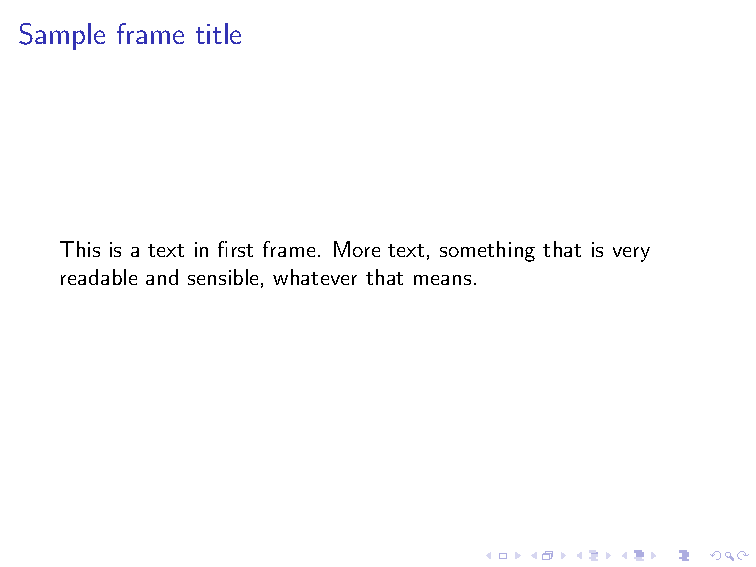
\includegraphics{IdentityTheftSlides/xdusek21-IdentityTheft.pdf}


\subsection{Příprava 3 -- Obecná bezpečnost na Internetu}
Příprava na hodinu s tématem \textbf{Obecná bezpečnost na Internetu} je rozdělena do několika částí:
\begin{itemize}
        \setlength{\itemsep}{-3pt}
        \item Specifikace tématu hodiny,
        \item stanovené cíle,
        \item náplň hodiny a časový plán,
        \item nutné pomůcky pro hodinu,
        \item text snímků prezentace.
\end{itemize}

\subsubsection{Specifikace tématu hodiny}
Tato hodina se zabývá aspekty obecné bezpečnosti z hlediska základního uživatelského používání internetového prohlížeče a interakce s webem jako takovým. Částečně téma této hodiny navazuje na předchozí hodinu zaměřenou na \textbf{Krádeže identity} - tato hodina se blíže zaměří na speciální případ krádeže identity, a to případ, kdy podvratná stránka napodobuje svým vzhledem vzhled stránky, kterou uživatel zná a věří ji. Tomuto specializované případu se taktéž říká \textit{Phishing}.

\subsubsection{Stanovené cíle}
Student zná a rozumím pojmům \textit{phishing}, \textit{vývojářská konzole} či jen \textit{konzole}, \textit{zdrojový kód}, \textit{http} a \textit{https}. Student umí rozlišit mezi bezpečnou webovou stránkou a stránkou, která se za bezpečnou webovou stránku pouze vydává. Student dovede posoudit, zda je přípustné do konkrétní webové stránky vyplňovat jakékoliv osobní informace. Student zná a umí vysvětlit problémy z hlediska bezpečnosti, které nastávají při využívání stránek bez podpory HTTPS (tedy stránek, které pro přenos informací mezi uživatelem a serverem využívají HTTP). Student ví k čemu slouží v prohlížeči tzv. \textit{vývojářká konzole} a uvědomuje si, rizika, které neuvážené kopírování a vkládání textu do ní může přinášet.

\subsubsection{Náplň hodiny a časový plán}
\indent\textbf{0. -- 3. minuta} - Zápis do třídní knihy. V případě, že výuka probíhá v počítačové učebně, zapnutí počítačů a přihlášení studentů do systému.

\textbf{4. -- 10. minuta} - Lehké představení tématu hodiny a odkázání se na hodinu týkající se \textbf{Krádeže identity}. Vyučující pokládáním otázek zjistí kolik si toho studenti ze zmíněné hodiny pamatují a nasměruje je na takové odpovědi, které povedou k tématu této hodiny. Například se může zeptat: \uv{Jaké si pamatujete, [Jméno Studenta], možné krádeže identit, ke kterým dochází?}, cílem je dovést studenty ke specializovanému případu krádeže identity, a to tomu případu, kdy se stránka vydává za jinou, uživateli známou stránku, což je přímo jedno z témat, které budou probrány.

\textbf{11. -- 25. minuta} - Vyučující využívající počítač připojený k Internetu a data projektoru spustí prohlížeč a ukáže studentům co je to vývojářská konzole a jakým způsobem je ji možné otevřít (tedy klávesou F12). Jsou-li studentům k dispozici počítače s nainstalovanými prohlížeči, vyučující jim pokyne, aby si to také ozkoušeli a vyřeší případné problémy studentů, kterým se konzoli nepodaří najít. Na náhodném webu pak studentům ukáže, jak se vepsání kódu do konzole na webu projeví - nejprve na jednoduchém příkladu (vyskakovací okénko), potom na složitějším (úprava obsahu stránky). Vysvětlí jim, že tyto změny se projevují pouze u něho v počítači; změny, které provede se nezobrazí dalším návštěvníkům stránky. Pro zvídavé studenty pak může zmínit, že jazyk, kterým se konzole ovládá, se jmenuje \textit{Javascript} a používá se hojně pro tvorbu webu. 

Studenti pravděpodobně touto dobou již vědí, že webové stránky jsou programovány a že existuje nějaký kód, na základě kterého jsou stránky zobrazovány. Vyučující toto pro jistotu připomene a ukáže studentům, jak je možné zdrojový kód stránek prohlížet (pro většinu prohlížečů klávesová zkratka \texttt{CTRL + U}). Při ukázce zdrojového kódu existující stránky studentům vysvětlí, že zkopírováním zdrojového kódu stránky a souvisejících souborů k sobě na webovou adresu, by došlo k vytvoření opticky shodné kopie webové stránky, která bude ovšem pod kontrolou někoho jiného. Vyučující se pak zeptá studentů, jestli si dovedou představit nějaký \uv{nepříjemný} scenář, ke kterému by mohlo takto dojít. Studenti by měli dojít k tomu, že by někdo mohl takto získávat informace od lidí, kteří si stránku spletou s originálem. Pokud na to studenti nedojdou, vyučující jim toto prozradí.

V tento moment také vyučující studentům popíše správný postup před zadáním jakýchkoliv soukromých či citlivých informací do webových stránek. Uživatel by měl \textbf{vždy} před vyplněním informací do stránky ověřit, že se opravdu nachází na stránce, na které předpokládá, že je. Toto ověření provede zkontrolováním adresního řádku v prohlížeči. Vyučující zmíní, že ne vždy musí být na první pohled zřejmé, že jde o závadnou stránku - velmi často jsou dnes používány názvy podobné názvu originálu. Jako konkrétní případ lze uvést stránku \textit{PayPal.com}, pro kterou existuje spousta podobných webových stránek, které se snaží napodobit originální jméno, aby působily důvěryhodně, například tedy \textit{PayiPal.com}, či \textit{PayPall.com}. Vyučující se dotáže studentů jaký by použili postup, pokud by si nebyli jistí, že jsou opravdu na stránce, na které chtějí být. Tato otázka může vést na vtipnou odpověď ze stran studentů ve způsobu \uv{Vygooglím si tu stránku?}, která bude v tomto případě na místě a pomůže uvolnit atmosféru v hodině.

Dalším vodítkem hodným zmínění je pak to, zda prohlížeč ve svém adresním řádku má před adresou webové stránky text \textit{https://} nebo \textit{http://}. Většina stránek velkých, středních, ale i menších organizací bude mít před adresou právě \textit{https://}. Většina podvodných stránek \textit{https://} mít vůbec nebude, nebo jen velmi krátkodobě. Vyučující vysvětlí studentům, že většina stránek má zájem o to mít \textit{https}, protože komunikace po tomto protokolu je šifrovaná a zaručuje, že po cestě nebude podvržena, napodobena, či zachycena. To znamená například, že při odesílání formuláře s přihlašovacími údaji na stránce bez aktivního \textit{https} spojení, je možné zachytit přihlašovací údaje po cestě mezi uživatelem a webovou stránkou; to na stránkách s aktivním \textit{https} spojením možné není, právě proto, že komunikace je šifrovaná.

\textbf{26. -- 40. minuta} - Vyučující se s využitím oporných snímků prezentace vrátí k vývojářské konzoli, se kterou studenty seznámil dříve v hodině. Na konkrétních případech skriptů, které byly v minulosti využívány k šíření spamu mezi uživateli sociální sítě Facebook, představí scénář, kterým je možné využít vývojářskou konzoli proti nic netušícímu uživateli. Vysvětlí scénář, který spočívá v přesvědčení uživatelů, že když nakopírují kód do své vývojářské konzole, odemknou si prémiovou verzi sociální sítě, která má lepší možnosti než ta stávající. Uživatelé, kteří kód nakopírují do konzole a pak spustí, můžou například nevědomě pozvat všechny své přátele k oblíbení si stránky, která patří útočníkovi, nebo můžou kompromitovat část svých citlivých dat. Vyučující představí reálné případy, kdy k podobným situacím došlo a varuje studenty, aby nikdy takto kód do konzole nekopírovali, pokud nevědí, co dělá. Bude-li čas a vhodná situace, vyučující může také jako zajímavost zmínit, že Facebook na tuto hrozbu reagoval a nyní při zobrazení vývojářské konzole v prohlížeči varuje uživatele, aby do ní nic nekopírovali.

\textbf{41. -- 45. minuta} - Shrnutí probrané látky a uzavření tématu. Vyučující dá prostor studentům pro otázky.

\subsubsection{Nutné pomůcky pro hodinu}
Pro efektivní realizaci výuky tak, aby bylo dosaženo stanových cílů je potřeba, aby vyučující měl k dispozici a počítač připojení k Internetu s data projektorem zobrazujícím obrazovku počítače třídě. Počítač by měl být vybaven dostatečně moderním internetovým prohlížečem, který obsahuje tzv. \textit{vývojářskou konzoli}.

\subsubsection{Text snímků prezentace}
Sem přijdou snímky prezentace k hodině.


\subsection{Příprava 4 -- Časté a zajímavé pojmy ze světa Kybernetické Bezpečnosti}
Příprava na hodinu s tématem \textbf{Časté a zajímavé pojmy ze světa Kybernetické Bezpečnosti} je rozdělena do několika částí:
\begin{itemize}
        \setlength{\itemsep}{-3pt}
        \item Specifikace tématu hodiny,
        \item stanovené cíle,
        \item náplň hodiny a časový plán,
        \item nutné pomůcky pro hodinu,
        \item text snímků prezentace.
\end{itemize}

Hodina je strukturována ve smyslu prezentace různých nepřímo souvisejících pojmů, se kterými se i běžný člověk, který s kybernetickou bezpečností nepřijde do styku na denní bázi, často setká. Na začátku hodiny je studentům představen seznam pojmů, které budou v hodině představeny a diskutovány. Následně jsou pak pojmy jeden po druhém postupně představovány, přičemž při každém přejití na nový pojem se vyučující dotazuje třídy, zda se s pojmem již setkali, popř. zda ho někdo ve třídě dokáže zjednodušeně vysvětlit. Tuto hodinu je možné zařadit na začátek celé výuky kybernetické bezpečnosti, kdy poslouží jako motivace studentů ke studiu a věnování se kybernetické bezpečnosti. Zároveň, pokud bude hodina podána vyhovující formou, může sloužit jako velmi lehký úvod do zajímavých aspektů kybernetické bezpečnosti, čímž může u studentů získat na popularitě. Další možností řazení hodiny je její umístění na konec vyučovacího roku, jako poslední zrelaxované a odlehčené téma pro třídu, které studentům dá podnět k vlastnímu studiu kybernetické bezpečnosti i dále - například během prázdnin před dalším během předmětu. Řazení na konec roku je výhodné v tom, že studenti již prošli celým předmětem, spoustu podstatných termínu znají a rozumí jim. A tedy je možné probrat v rámci této hodiny i více komplexní a zajímavá témata, popřípadě provést důkladnou diskuzi na téma.

\subsubsection{Specifikace tématu hodiny} 
Hodina se tématicky zabývá vzájemně nepřímo souvisejícími termíny z oblasti kybernetické bezpečnosti. Pojmy probírané v hodině jsou vybrány tak, aby většinu z nich studenti již za svůj život slyšeli a tato hodina jim pomohla tyto termíny správně uchopit. Probírané termíny jsou pak také vybírány na základě jakési \uv{popularity}, neb mají ve studentech vzbudit zvědavost a určitý pocit senzace, mají na ně působit zajímavě a tajemně. Tato konkrétní příprava na hodinu se zabývá tématem útoků v síti internetu DoS a DDoS, sociálním inženýrstvím, anonymním pohybem po Internetu, sítí TOR a \textit{Deep Webem}. Probrán je také termín botnet. V reálné situaci by však tato příprava na hodinu měla být připravena s ohledem na aktuální důležité termíny a události, které se v oblasti kybernetické bezpečnosti dějí v době očekávaného výkladu, aby poskytnuté informace byly dostatečně aktuální a zajímavé.


\subsubsection{Stanovené cíle}
Student rozumí pojmům DoS a DDoS útok a dovede vysvětlit rozdíl mezi nimi. Student zná pojem \uv{sociální inženýrství} a uvědomuje si jeho rizika a právní závadnost případné aplikace jeho disciplín. Student ví, co je to \textit{TOR} a k čemu slouží. Student ví jakým způsobem je možné přistoupit na tzv. \uv{\textit{Deep Web}}, a co je na něm možné nalézt. Uvědomuje si, že samotný přístup na \textit{Deep web} není trestný, avšak vyhledávání a prohlížení materiálů, které jsou v rozporu se zákony země, ve které žije, může způsobit právní problémy. Student rozumí pojmu botnet a zná nějaké historicky obrovské botnety a jejich roli ve světě. 
 

\subsubsection{Náplň hodiny a časový plán}
\indent\textbf{0. -- 3. minuta} - Zápis do třídní knihy. V případě, že výuka probíhá v počítačové učebně, zapnutí počítačů a přihlášení studentů do systému.

\textbf{4. -- 8. minuta} - Vyučující promítne na data projektoru úvodní snímek prezentace, na kterém jsou pod sebou v seznamu vypsané termíny, o kterých plánuje v hodině mluvit. Pokyne studentům, aby si zběžně přečetli seznam a dá jim na to trochu času. Následně studentům prozradí, že o těchto pojmech budou tuto hodinu mluvit, a že nyní bude číst pojmy jeden po druhém a pokud někdo ve třídě tento pojem již slyšel, zvedne ruku. Vyučující pak na základě počtu rukou, které zůstávají dole, detekuje nejméně obecně známý pojem a bude vědět, na který termín si má vyhradit nejvíce a naopak nejnémě času. Dle situace a času může vyučující pobídnout někoho ze třídy, aby pojem lehce osvětlil zbytku třídy, bude-li chtít.

\textbf{9. -- 35. minuta} - V tomto časovém úseku budou vysvětlovány a diskutovány jednotlivá témata a termíny, kterými se hodina zabývá. V rámci přípravy je to řazeno do jednoho dlouhého časového úseku, neb se očekává, že vyučující bude pracovat s časem během hodiny dynamicky - dle znalostí třídy, řazení této hodiny a rozsáhlosti diskusí a studentských dotazů k jednotlivým probíraným tématům.

Vyučující začne přepnutím snímku prezentace na snímek o DoS a DDoS útocích. Vysvětlí studentům anglický význam a překlad těchto zkratek (\textit{Denial of Service}, \textit{Distributed Denial of Service}). Vyučující objasní studentům, že tento populární útok je založen na nárazovém mnohonásobném připojení více klientů / instancí klientů na server za účelem vytížení serveru a znemožnění přístupu legitimních klientů. Po vysvětlení základního princpu a významu zkratek se vyučující pokusí společně se třídou dojít metodou pokládání vhodných otázek k zásadnímu rozdílu mezi útoky. Studenti by měli dojít k uvědomění, že \textit{DDoS} útok je založený na větším množství klientů, rozmístěných například po celém světe, kteří naráz provádějí \textit{DoS} útok. Nedojdou-li k tomu studenti sami od sebe, bude jim to vyučujícím prozrazeno.

Plynulým navázáním na tyto často se vyskytující typy útoků se vyučující přesune k další, pro studenty jistě velmi zajímavé oblasti - vyvětlení, jak principielně může probíhat útok, při kterém se útočník na stejné síti (například. wifi) dostane na počítač oběti útoku. Společně s otevřením tohoto tématu se vyučující posune na odpovídající snímek své prezentace. Popíše jeden z možných scénářů, kterým by útok mohl proběhnout, aby studentům principielně přiblížil, jak to reálně celé probíhá, a to aby konkretizoval představu o tom, co to znamená, když se řekne, že \uv{útočníci se hacknuli do počítače [jméno napadeného člověka]}. Bodově půjde o vysvětlení, že útočník si nejprve provede \uv{průzkum} v rámci kterého nějakým způsobem \uv{proskenuje} síť. Skenováním sítě je myšleno zjištění, jaká zařízení jsou v síti na jakých adresách. Jakmile zjistí útočník zařízení v síti, skenuje pak přímo jednotlivě ty. Útočník se pokusí zaslat zprávy na konkrétní zařízení a podle způsobů, kterým zařízení odpovídají, někdy dokáže určit, jaký operační systém a v jaké verzi na strojích běží, popřípadě někdy i jaké programy. Dalším krokem je pak to, že útočník nalezne způsob, jak operační systém nebo běžící program zneužít tak, aby mu byl udělen přístup k zařízení. Toto probíhá typicky tak, že vyhledá v databázi známých bezpečnostních problémů problém konkrétního programového vybavení, které běží na zařízeních v síti. Tohoto bezpečnostního problému dále využije k tomu, aby zařízení napadl a převzal nad ním kontrolu.

Dále se vyučující posune na snímek prezentace týkající se sociálního inženýrství. Nejprve se studentů zeptá, co si pod tímto pojmem představí, když ho teď slyší, aby získal představu o tom, jak dalece třída ví o co se jedná. Po úvodních námětech z třídy se dostane vyučující k představení tématu sociálního inženýrství. Vysvětlí třídě, že lidé, kteří jsou nazývání sociálními inženýry, jsou specialisté v získávání informací o lidech, procesech, firmách a dalších možných entitách. Obvykle jde o cenné informace buď přímo pro ně, nebo pro osobu, pro kterou pracují. K získávání těchto informací využívají různých manipulačních technik a postupů, ve kterých jsou velmi zběhlí. Vysvětlí, že sociální inženýři velmi často využívají toho, že lidé považují spoustu informací za nepodstatnou a bez problému ji mimoděk sdělí okolí. Pro ilustraci toho, jaký dopad mohou mít zdánlivě nepodstatné informace na společnost nebo profit jednotlivce, sociálního inženýra, představí vyučující příběh nejmenovaného sociálního inženýra z knihy \textit{The Art of Deception}, od Kevina D. Mitnicka, který demonstruje, jakým způsobem jednoduché, bezcenné informace lze využít. V konkrétním případě volal člověk na několik linek bankovní společnosti, aby nejprve zjistil jakým správným způsobem se ve firmě nazývají určité procedury a informace. Pod záminkou psaní knihy zjistil nejprve to, jak se správně říká \textit{identifikátoru obchodníka}, který se používá u americké firmy \textit{CreditChex} k ověření, že volající co má zájem o informace, volá ze správné firmy. Poděkoval za informaci a vytočil číslo banky, ze které dostal identifikátor obchodníka a volal s jinou operátorkou. Té se představil jako zástupce firmy \textit{CreditChex}, který provádí vyhodnocování spokojenosti klientů jejich firmy a vyptal se operátorky na několik otázek zdánlivě souvisejících se zjišťováním její spokojenosti. Mezi tyto otázky vložil dotaz na identifikátor obchodníka, který používají. Operátorka, považující tuto informaci za naprosto bezcennou, bez váhání sociálnímu inženýrovi tuto informaci sdělila. Co efektivně sociální inženýr během těchto dvou hovorů získal, pak byla možnost nyní volat do \textit{CreditChex} společnosti a využívat jejich služeb, aniž by za ně musel platit (nemluvě o tom, že běžní smrtelníci k těmto informacím ani přístup jednoduše nezískají).

Další téma hodiny se týká anonymizační sítě \textit{TOR} a přístupu na \textit{Deep Web}. S vysokou pravděpodobností půjde o - pro studenty - nejzajímavější část hodiny. Vyučující se opět posune na snímek a vysvětlí studentům, že v rámci této hodiny nemá v úmyslu vysvětlovat jim, jak anonymizační síť TOR přesně funguje, ale chce jim objasnit, k čemu je dobrá, jak ji využívat a co se na ní dá všechno najít. Vyučující třídě představí \textit{TOR} jako způsob, kterým může kdokoliv na Internetu při správném používání zakrýt svou identitu, což znamená, že když osoba využívající \textit{TOR}, přistoupí na jakoukoliv webovou stránku, nikdo by neměl být schopen detekovat, že se tak stalo, dokonce by ani nemělo být možné zjistit, z jaké země se člověk připojil. Zde také studentům vysvětlí, že toto platí pouze za předpokladu, že studenti nejsou při používání služeb sítě \textit{TOR} připojeni do svých Facebookových, mailových či jiných účtů, které uchovávají informace o jejich reálné identitě. Následně se studentů zeptá, jaké si dovedou představit scénáře, kdy by uživatel mohl mít zájem na skrytí své identity na Internetu. Dá se očekávat, že studenti přijdou s důvody, které se odkazují na často pochybné, i nelegální chování. Vyučující by je měl nabádat, aby našli i legitimní důvody, proč by člověk chtěl zůstat na Internetu anonymní. Pokud studenti nepřijdou se svými důvody, řekne jim, že například spousta žurnalistů potřebuje zůstat na Internetu při získávání informací nebo publikování v anonymitě, aby se nestali terčem útoku, pokud budou psát o něčem, co se někomu nebude líbit. Dalšími případy by pak mohli být lidé skrývající se před všude přítomnou personalizovanou reklamou.

Vyučující studentům představí nejjednodušší, avšak nejméně bezpečný způsob, jak využívat \textit{TOR} k anonymnímu prohlížení Internetu - tento fakt nezapomene zmínit. Způsobem připojení se je využití modifikovaného prohlížeče \textit{Firefox}, který se umožňuje připojit k \textit{TOR} síti. IP adresa, ze které pak uživatel navštěvuje weby, není jeho vlastní, ale náhodného uzlu připojeného v anonymizační síti. Vyučující studentům vysvětlí výhody a nevýhody anonymního přístupu na Internet prostřednictvím sítě \textit{TOR}. V tento moment studentům také přiblíží pojem \textit{Deep Web}, který referuje na stránky, jež nejsou přístupné z běžného Internetu a dostane se k nim člověk pouze, pokud je připojen k \textit{TOR} síti. Tyto stránky mají koncovku \texttt{.onion} a běžně mívají, v závislosti na jejich (ne)legalitě i náhodné jméno složené z alfa numerických znaků (tj. znaků a-z a čísel). Vyučující studentům řekne, co všechno za stránky se dá nalézt - od obchodů se zbraněmi, drogami či vraždami, až po zcela normální webové stránky, které se pouze z důvodu jakési \uv{senzace} skrývají za \textit{TOR}em. V tento moment je studentům také sděleno, že samotné navštěvování webu přes TOR není nijak trestně závadné, avšak pokud se budou pohybovat po stránkách jejiž obsah je v rozporu s právy v zemi, ve které žijí, můžou být právně postihování, pokud tato skutečnost vyjde najevo. Toto varování patří například ke stránkám, na kterých může docházet k obchodování s drogami, zbraněmi, lidmi, nebo dětskou pornografií.

Posledním tématem k probrání jsou \textit{botnety}. Vyučující opět začne tento blok posunem na nový snímek a dotazem studentů, jestli by někdo z nich dovedl popsat, co to botnet je. Výsledkem společné práce vyučujícího se studenty by mělo být uvědomění studentů, že botnet je skupina zařízení, typicky připojených k Internetu, která po nějakém kanálu přijímají pokyny od majitele botnetu. Příkladem příkazu, který může vydat majitel botnetu je, aby se všechny zařízení připojené v botnetu připojovala opakovaně na nějakou webovou stránku. V tento moment se vyučující zeptá, zda to studentům připomíná nějaké z témat, o kterém se v této hodině mluvilo. Očekávanou odpovědí jsou DoS a DDoS útoky, přičemž DDoS je více vítaná odpověď, neb díky většímu počtu reálných klientů po světě jde o distribuovaný útok na dostupnost služby. Dále se vyučující zeptá studentů, jaká všechna zařízení si myslí, že se mohou připojovat do botnetů. Vzhledem k rapidnímu rozvoji fenoménu zvaného \textit{IoT (Internet of Things)}, je správnou odpovědí i široká odpověď jako \uv{Potenciálně jakékoliv zařízení s připojením na Internet}. Konkrétně to však v době psaní této práce jsou počítače, telefony, notebooky, chytré ledničky a vysavače, auta apod.

\textbf{40. -- 45. minuta} - Zopakování důležitých termínu z probrané hodiny a shrnutí probrané látky.

\subsubsection{Nutné pomůcky pro hodinu}
Pro splnění cílů hodiny mimořádně není nutné žádné speciální elektronické vybavení. Celou hodinu je možné odvést a odvykládat ve standardní učebně, avšak vyučující může benefitovat z dostupnosti počítače napojeného na data projektor. Počítač s data projektorem může využít k živým ukázkám vykládané látky a promítání textů a obrázků na snímcích oporné prezentace. Není-li počítač s data projektorem k dispozici, obsah snímků prezentací lze vyměnit za tabuli a fix, popřípadě křídu.

\subsubsection{Text snímků prezentace}




% SECTION CONCLUSION
\newpage
\section{Závěr}
V této práci byl navržen možný způsob implementace výuky kybernetické bezpečnosti do výuky předmětu \textit{Informatika a ICT}, který je vyučován na gymnáziích. Implementace je realizována rozšířením obecně používaného modele výuky předmětu \textit{Informatika a ICT}. Výuka je rozšířena ze dvou hodin týdně během prvních dvou let na 3 hodiny, kde přidaná hodina je věnována výuce kybernetické bezpečnosti navazující na probrané téma v hodinách standardní informatiky. Dále je rozšiřována výuka informatiky jako takové do třetího a čtvrtého ročníku s dotací 2 hodin týdně. Jedna hodina je věnována probírání nového tématu z oblasti informačních technologií a jedna opět na navazující bezpečnostní aspekty nově probírané oblasti.

Před samotnou realizací cíle této práce byl prostudován RVP pro gymnázia v jehož obsahu byly vyznačeny body pod než by výuka kybernetické bezpečnosti mohla rámcově spadat. Dále bylo navrženo a argumentováno možné rozšíření RVP pro výuku informatiky o nový tématický celek vyhrazený speciálně pro kybernetickou bezpečnost.

Následně jsou v této práci vymezeny \textit{vstupní dovednosti}, které by student před započetím studia kybernetické bezpečnosti měl zvládat, \textit{nutné pomůcky} pro výuku a navržen \textit{časový rozvrh výuky napříč ročníky}. Představeny jsou také metody a formy výuky autorem této práce uvažované za vhodné pro předmět kybernetické bezpečnosti.

Zhotoven byl taktéž \textit{tématický plán}, který představuje témata učiva rozdělené do čtyř let výuky předmětu \textit{Informatika a ICT} rozšířeného o výuku kybernetické bezpečnosti. Zaváděny jsou témata cílená na praktické využití studenty ještě během studií, ale i s prospekty na budoucí úplatnění v praxi, rozhodnou-li se pronásledovat kariéru v oblasti informačních technologií nebo kybernetické bezpečnosti. Očekávaným případem použití tématického plánu je jeho využití učitelem informatiky k přípravě učebních plánů pro výuku v konkrétním roce.

V poslední kapitole jsou pak uvedeny 4 přípravy do hodiny, které ukazují jakým způsobem by mohla probíhat výuka hodin kybernetické bezpečnosti. Přípravy na hodiny jsou doplněny o snímky prezentace, která by očekávatelně byla použita při vyučovací hodině.

% === REFERENCES & LITERATURE ===
\newpage
\begin{thebibliography}{9}

    \bibitem{malwareUnicornAppretince}
    Selena Larsen: Malware researcher helps teen hackers turn skills into careers,
    \\\textit{http://money.cnn.com/2017/07/12/technology/malware-researcher-helps-teen-hackers}.

    \bibitem{waveRVP}
    Národní Ústav pro Vzdělávání: Přehled vydávání RVP SOV po vlnách,
    \\\textit{http://www.nuv.cz/t/prehled-vydavani-rvp-sov-po-vlnach}.

    \bibitem{rvpGym}
    \textit{Rámcový vzdělávací program pro gymnázia}. [online]. Praha: VÚP, 2007. [cit. 2017-09-09]. Dostupné z WWW: $<$http://nuv.cz/file/159$>$.

    \bibitem{rvpElementary}
    \textit{Rámcový vzdělávací program pro základní vzdělávání}. [online]. Praha: MSMŠT, 2017. [cit. 2017-09-09]. Dostupné z WWW: $<$http://www.nuv.cz/uploads/RVP\_ZV\_2017\_verze\_cerven.pdf$>$.

    \bibitem{svpGymbos}
    \textit{Školní vzdělávací program: Kráčíme k maturitě. Non scholae, sed vitae discimus (Neučíme se pro školu, ale pro život)}. [online]. Gymnázium Boskovice. [cit. 2017-09-09]. Dostupné z WWW: $<$http://www.gymbos.cz/dokumenty/SVP-VG-GB.pdf$>$


    \bibitem{presentationPavlaZ}
    ZIELENIECOVÁ, Pavla. \textit{Příprava učitele na výuku. Vzdělávání učitelů.} [online prezentace]. Praha: Katedra didaktiky fyziky, Matematicko-fyzikální fakulta, UK, 2015, [cit. 2017-19-08]. Dostupný z WWW: $<$https://kdf.mff.cuni.cz/vyuka/pedagogika/materialy/2015\%20ZS/8\%20Priprava\\\%20ucitele\%20na\%20vyuku.\%20Legislativni\%20zakotveni\%20ucitele.pdf$>$.

\end{thebibliography}
\end{document}



% DRAFT LEFTOVERS
% I am very sad about removing the following paragraphs 
% Na následujících stránkách jsou popsány dva možné tématické plány výuky kybernetické bezpečnosti na gymnáziích. První tématický plán uvažuje možnost výuky kybernetické bezpečnosti v rámci výuky hodin informačních technologí po její celou dobu stanovenou školou. Druhý tématický plán je realizován s předpokladem, že například v rámci 3. a 4. ročníku, je pro výuku kybernetické bezpečnosti dedikován samostatný předmět.
% V rámci prnvího tématického plánu má výuka kybernetické bezpečnosti sloužit jako \textit{rozšíření} nebo \textit{doplnění}, které je možné vložit do standardní výuky informatiky realizované na gymnáziích. 
% V případě druhého plánu, narozdíl od výuky kybernetické bezpečnosti v rámci výuky informatiky umožňuje studentům se přímou soustředit a profilovat v oblasti kybernetické bezpečnosti. Další výhodou takovéto výuky je možnost podání látky v nahuštěnější formě, s vyšším důrazem na konkrétní problémy a jejich správné uchopení. V případě dedikovaného předmětu se není nutné vázat na probírané oblasti ve výuce standardní informatiky, ale je možné se věnovat konkrétním problémům kybernetické bezpečnosti a jejich řešení. Profilování se studentů v oblasti kybernetické bezpečnosti pro ně v dnešní době může být obzvláště zajímavé, neb se očekává, že rokem 2023 bude nedostatek kvalifikovaných specialistů v oblasti kybernetické (a informační) bezpečnosti.
%excerpt:některými častými útoky na webové aplikace, 
%excerpt:Student umí vyjmenovat a bez zabíhání do detailů přiblížit alespoň 2 časté útoky na webové aplikace.
%Dalším tématem k rychlému probrání je časté téma napadání webových stránek. Vyučující v naprosté rychlosti představí dva přístupy - jeden jehož výsledkem je vložení nežádoucího zdrojového kódu do webových stránek a druhý, který je postaven na prohledávání a práci s připojenou databází k webové stránce takovým způsobem, který autor stránky nezamýšlel. U prvního zmiňovaného útoku vyučující předpokládá, že žáci již vědí, že webové stránky jsou psány za pomocí HTML, CSS a Javascript technologií. Tento předpoklad však ještě ověří. Dojde-li k závěru, že větší část třídy nemá představu o tom, jak webové stránky vznikají a fungují, nemá smysl se útoky na webové aplikace zabývat a tato část bude přeskočena.
%Má-li třída představu o tom, jak webové stránky fungují, vyučující objasní, že první typ útoku se jmenuje XSS, u kterého rozlišujeme dva případy -- \textit{reflektovaný} a \textit{ukládaný}. Rozdíl mezi nimi je způsob, kterým se útočníkův zdrojový kód do stránek dostává. Při reflektovaném útoku ho stránka do sebe vypisuje na základě informací obdržených od uživatele (například z adresy při odesílání formuláře, nebo z vyhledávacího políčka). 
%Červenec &
%    Internet (3x) \newline
%    Bezpečnostní aspekty tématu Internet (1x) \newline
%    Bezpečnostní aspekty tématu Počítačové sítě (1x) \newline
%    6 \newline 1 \newline 1 \newline 1
%\\ \hline
%Červenec &
%    Používání relačních databází (1x) \newline
%    Algoritmizace (1x) \newline
%    Bezpečnost webových aplikací a databází (2x) &
%    2 \newline 2 \newline 2
%    \\ \hline
% \subsubsection{Metoda výuky: Didaktická hra - Celoroční tématika}
% TODO: Hra co má probíhat celý rok a přinášet studentům body.